% !TeX program = xelatex
\documentclass[12pt,a4paper]{article}

\usepackage{fontspec}
\usepackage[russian]{babel}
\setmainfont{DejaVu Serif}
\setsansfont{DejaVu Sans}
\setmonofont{DejaVu Sans Mono}
\usepackage{geometry}
\usepackage{indentfirst}
\usepackage{setspace}
\usepackage{enumitem}
\usepackage{array}
\usepackage{longtable}
\usepackage{tabularx}
\usepackage{booktabs}
\usepackage{graphicx}
\usepackage{float}
\usepackage{xcolor}
\usepackage{tikz}
\usepackage[hidelinks]{hyperref}

\usetikzlibrary{arrows.meta,positioning,shapes.geometric,fit,calc}
\geometry{left=2.5cm,right=1.5cm,top=2cm,bottom=2cm}
\onehalfspacing
\setlength{\parindent}{1.25cm}
\setlength{\parskip}{0pt}
\setlist{nosep,leftmargin=1.25cm}
\renewcommand{\arraystretch}{1.25}
\sloppy

\definecolor{itmoblue}{RGB}{27,74,132}
\definecolor{lightblue}{RGB}{232,240,249}
\definecolor{lightgray}{RGB}{245,245,245}

\newcommand{\systemname}{«ЛабРезерв»}
\newcommand{\req}[1]{\textbf{#1}}
\newcommand{\uc}[1]{\textbf{#1}}

% Сценарии прецедентов оформляются построчно: каждый шаг визуально отделён.
\newlist{ucsteps}{enumerate}{1}
\setlist[ucsteps]{label=\arabic*),leftmargin=*,itemsep=5pt,topsep=4pt,parsep=0pt}
\newlist{ucalts}{enumerate}{1}
\setlist[ucalts]{label=A\arabic*:,leftmargin=*,itemsep=5pt,topsep=4pt,parsep=0pt}

\begin{document}
\hypersetup{pageanchor=false}
\pagenumbering{gobble}

\begin{titlepage}
\begin{center}
    \large
    Национальный исследовательский университет ИТМО\\
    Факультет программной инженерии и компьютерной техники\\
    \vspace{2.5cm}
    \textbf{\Large Информационные системы}\\
    \vspace{0.5cm}
    \textbf{\Large Отчёт по курсовой работе}\\
    \vspace{0.35cm}
    \textbf{\large Этап 1}\\
    \vspace{0.8cm}
    \textbf{\Large Система управления бронированием\\
    и загрузкой оборудования в лаборатории/цеху}\\
    \vspace{2.4cm}
    \begin{flushright}
        Выполнили студенты 3 курса:\\
        Калинин Дмитрий Викторович\\
        Рзаев Ахмед Меджидович\\
        \vspace{0.6cm}
        Преподаватель:\\
        Николаев Владимир Вячеславович
    \end{flushright}
    \vfill
    Санкт-Петербург, 2026
\end{center}
\end{titlepage}

\clearpage
\hypersetup{pageanchor=true}
\pagenumbering{roman}
\begin{singlespace}
\tableofcontents
\end{singlespace}
\newpage
\pagenumbering{arabic}

\section{Введение}

Цель курсовой работы --- спроектировать информационную систему для управления
бронированием и фактической загрузкой оборудования учебной лаборатории,
мастерской или производственного цеха. На первом этапе определяются границы
предметной области, назначение системы, требования, основные прецеденты и
архитектура будущего программного решения.

Рабочее название системы --- \systemname. Ключевая особенность системы состоит
в автоматическом разрешении конфликтов: если оборудование занято, находится на
техническом обслуживании или неисправно, система не ограничивается отказом, а
подбирает допустимые альтернативы по времени и по функционально эквивалентному
оборудованию.

\section{Описание предметной области}

\subsection{Объект автоматизации}

Объектом автоматизации является подразделение, располагающее ограниченным
парком дорогостоящего или уникального оборудования. Это может быть учебная
лаборатория, конструкторское бюро, мастерская или производственный цех. В состав
парка могут входить 3D-принтеры, лазерные резаки, станки с ЧПУ, измерительные
приборы и испытательные стенды.

Одними и теми же единицами оборудования пользуются разные сотрудники, студенты
и учебные группы. Для безопасной работы пользователь должен иметь действующий
допуск к соответствующему типу оборудования. Оборудование периодически
недоступно из-за планового технического обслуживания, а также может быть
выведено из эксплуатации вследствие внеплановой неисправности.

\subsection{Участники предметной области}

Участниками предметной области являются люди, которые непосредственно участвуют
в процессах использования и обслуживания оборудования. Информационная система не
рассматривается как самостоятельный участник предметной области: её поведение и
ответственность фиксируются функциональными и нефункциональными требованиями.

\begin{longtable}{|p{0.25\textwidth}|p{0.65\textwidth}|}
\hline
\textbf{Участник} & \textbf{Ответственность} \\
\hline
\endfirsthead
\hline
\textbf{Участник} & \textbf{Ответственность} \\
\hline
\endhead
Пользователь & Просматривает доступное оборудование, создаёт и отменяет
бронирования, выбирает предложенную альтернативу, отмечает начало и окончание
работы, сообщает о неисправности. \\
\hline
Администратор лаборатории & Ведёт каталог оборудования и типов оборудования,
назначает и отзывает допуски, контролирует расписание, фиксирует неисправности,
анализирует загрузку. \\
\hline
Техник (инженер по обслуживанию) & Планирует и выполняет техническое
обслуживание, фиксирует результаты ремонта и изменяет техническое состояние
оборудования. \\
\hline
\end{longtable}

\subsection{Основные информационные объекты}

В системе обрабатываются сведения о пользователях и их ролях, типах и единицах
оборудования, функциональных возможностях оборудования, допусках, бронированиях,
периодах технического обслуживания, неисправностях и ремонтах, фактических
сеансах использования, предложенных альтернативах и уведомлениях. Для каждой
операции, влияющей на доступность оборудования, должна сохраняться история.

\subsection{Текущее состояние и проблемы}

Без специализированной системы расписание обычно ведётся в бумажном журнале,
электронной таблице или формируется устными договорённостями. Такой процесс не
гарантирует актуальность данных и приводит к следующим проблемам:

\begin{itemize}
    \item одно оборудование бронируется несколькими пользователями на
    пересекающиеся интервалы;
    \item бронирование назначается на период планового обслуживания;
    \item пользователь получает доступ к оборудованию без необходимого допуска;
    \item после поломки все последующие бронирования приходится переносить
    вручную;
    \item участники поздно узнают об изменениях расписания;
    \item плановая загрузка не сопоставляется с фактическим временем работы;
    \item отсутствуют достоверные данные для решений о закупке и обслуживании.
\end{itemize}

\subsection{Бизнес-правила и ограничения}

\begin{enumerate}[label=BR-\arabic*.]
    \item Бронирование может создать только активный пользователь с действующим
    допуском к выбранному типу оборудования.
    \item Временные интервалы подтверждённых бронирований одной единицы
    оборудования не должны пересекаться.
    \item Бронирование не может пересекать период технического обслуживания или
    недоступности из-за неисправности.
    \item Время окончания любого интервала должно быть позже времени начала.
    \item Альтернативная единица оборудования должна поддерживать требуемую
    функцию, быть доступной и соответствовать допуску пользователя.
    \item Приоритет альтернатив: тот же станок в ближайшее время; затем
    эквивалентный станок в исходное время; затем эквивалентный станок в ближайшее
    время.
    \item Назначение обслуживания или регистрация поломки переводит затронутые
    будущие бронирования в состояние «требует переноса», но не переносит их без
    выбора пользователя или администратора.
    \item Завершённые и отменённые бронирования не изменяются; исправления
    выполняются отдельной записью аудита.
    \item Фактический сеанс использования может быть открыт только для
    подтверждённого бронирования и закрывается ровно один раз.
    \item Все моменты времени хранятся с часовым поясом; в интерфейсе
    отображается часовой пояс лаборатории.
\end{enumerate}

\section{Назначение и задачи системы}

\subsection{Назначение}

Система предназначена для формирования единого достоверного расписания
оборудования, предотвращения конфликтов доступа и сокращения ручной работы при
изменении доступности. Она должна обеспечить безопасное использование техники
с учётом допусков и предоставить администрации данные о реальной загрузке
парка.

\subsection{Решаемые задачи}

\begin{enumerate}
    \item Централизованно учитывать оборудование, его характеристики,
    функциональные возможности и текущее состояние.
    \item Учитывать квалификацию и допуски пользователей.
    \item Создавать непротиворечивое расписание бронирований.
    \item Автоматически блокировать периоды планового обслуживания и ремонта.
    \item Подбирать варианты переноса при конфликте, обслуживании или поломке.
    \item Уведомлять пользователей об изменении состояния их бронирований.
    \item Фиксировать фактическое начало и окончание работы.
    \item Рассчитывать показатели загрузки, конфликтности и простоев.
\end{enumerate}

Ожидаемый эффект --- уменьшение числа сорванных работ и времени администратора
на согласование расписания, повышение прозрачности причин простоя и получение
данных для обоснованного планирования закупок.

\section{Требования к информационной системе}

\subsection{Функциональные требования}

Функциональные требования сгруппированы по связанным областям ответственности,
чтобы требования одного бизнес-процесса рассматривались совместно.

\begin{longtable}{|p{0.11\textwidth}|p{0.79\textwidth}|}
\hline
\textbf{Код} & \textbf{Требование} \\
\hline
\endfirsthead
\hline
\textbf{Код} & \textbf{Требование} \\
\hline
\endhead
\multicolumn{2}{|l|}{\textbf{Аутентификация, каталог оборудования и допуски}} \\
\hline
\req{FR-01} & Система должна обеспечивать аутентификацию и разграничение
действий по ролям пользователя, администратора и техника. \\
\hline
\req{FR-02} & Администратор должен иметь возможность создавать, изменять,
архивировать типы и единицы оборудования, указывая характеристики и функции. \\
\hline
\req{FR-03} & Система должна хранить состояние оборудования: доступно,
обслуживание, неисправно, архивировано. \\
\hline
\req{FR-04} & Администратор должен назначать и отзывать допуски с указанием
типа оборудования, срока действия и основания. \\
\hline
\req{FR-05} & Пользователь должен просматривать каталог и календарь доступности
оборудования. \\
\hline
\multicolumn{2}{|l|}{\textbf{Бронирование и разрешение конфликтов}} \\
\hline
\req{FR-06} & Пользователь должен создавать заявку на бронирование, указав
оборудование или требуемую функцию, начало, окончание и цель работы. \\
\hline
\req{FR-07} & До подтверждения система должна проверить допуск, состояние
оборудования, пересечения с бронями и техническим обслуживанием. \\
\hline
\req{FR-08} & При успешной проверке система должна создать подтверждённое
бронирование атомарно, исключая одновременное занятие слота другим запросом. \\
\hline
\req{FR-09} & Пользователь должен отменять своё будущее бронирование с
фиксацией времени и причины отмены. \\
\hline
\req{FR-10} & При конфликте система должна искать ближайшие свободные слоты на
том же оборудовании в пределах настраиваемого горизонта поиска. \\
\hline
\req{FR-11} & Система должна искать оборудование с требуемой функцией, проверяя
его доступность и допуск пользователя. \\
\hline
\req{FR-12} & Система должна ранжировать и предъявлять пользователю не менее
трёх альтернатив, если столько допустимых вариантов существует. \\
\hline
\req{FR-13} & Пользователь должен подтверждать одну альтернативу; перед
сохранением система обязана повторно проверить её актуальность. \\
\hline
\multicolumn{2}{|l|}{\textbf{Плановое обслуживание, неисправности и ремонт}} \\
\hline
\req{FR-14} & Техник должен создавать, изменять и отменять периоды планового
технического обслуживания. \\
\hline
\req{FR-15} & При назначении обслуживания система должна определить все
пересекающиеся будущие бронирования и инициировать для них подбор альтернатив. \\
\hline
\req{FR-16} & Пользователь, администратор или техник должен зарегистрировать
неисправность с описанием; перевод оборудования в состояние «неисправно»
доступен администратору и технику. \\
\hline
\req{FR-17} & При поломке система должна выявить затронутые бронирования,
сформировать альтернативы и уведомить их владельцев. \\
\hline
\req{FR-18} & Техник должен фиксировать ремонт и возвращать оборудование в
состояние «доступно» после проверки. \\
\hline
\multicolumn{2}{|l|}{\textbf{Фактическое использование оборудования}} \\
\hline
\req{FR-19} & Пользователь должен отмечать фактическое начало и завершение
работы по бронированию. \\
\hline
\req{FR-20} & Система должна хранить плановую и фактическую продолжительность
использования раздельно. \\
\hline
\multicolumn{2}{|l|}{\textbf{Уведомления, аналитика и аудит}} \\
\hline
\req{FR-21} & Система должна создавать внутрисистемные уведомления об отмене,
переносе, приближении бронирования и изменении состояния оборудования. \\
\hline
\req{FR-22} & Администратор должен получать отчёт по утилизации оборудования,
частоте конфликтов и длительности простоев за выбранный период. \\
\hline
\req{FR-23} & Администратор должен фильтровать и выгружать аналитический отчёт
в CSV. \\
\hline
\req{FR-24} & Система должна вести журнал значимых действий: изменение
оборудования, допусков, бронирований, обслуживания и технического состояния. \\
\hline
\end{longtable}

\subsection{Нефункциональные требования}

Нефункциональные требования сгруппированы по качественным характеристикам системы
и эксплуатационным ограничениям.

\begingroup
\small
\setstretch{1.25}
\renewcommand{\arraystretch}{1.05}
\begin{longtable}{|p{0.11\textwidth}|p{0.79\textwidth}|}
\hline
\textbf{Код} & \textbf{Требование и критерий проверки} \\
\hline
\endfirsthead
\hline
\textbf{Код} & \textbf{Требование и критерий проверки} \\
\hline
\endhead
\multicolumn{2}{|l|}{\textbf{Производительность}} \\
\hline
\req{NFR-01} & Время ответа для 95\% операций просмотра каталога и календаря
не должно превышать 2 секунд при 100 одновременных пользовательских сессиях. \\
\hline
\req{NFR-02} & Подбор альтернатив должен завершаться не более чем за 5 секунд
при каталоге до 1000 единиц и горизонте поиска 30 дней. \\
\hline
\multicolumn{2}{|l|}{\textbf{Целостность и конкурентный доступ}} \\
\hline
\req{NFR-03} & Операция подтверждения бронирования пользователя должна быть транзакционной:
при конкурентных запросах подтверждается не более одного пересекающегося
бронирования. \\
\hline
\multicolumn{2}{|l|}{\textbf{Безопасность, авторизация и аудит}} \\
\hline
\req{NFR-04} & Пароли должны храниться в виде хешей Argon2id с уникальной солью
не короче 16 байт и параметрами $m \geq 19$ МиБ, $t \geq 2$, $p \geq 1$.
Внешний обмен --- только по HTTPS с TLS 1.2 или выше; SSL и более ранние версии
TLS должны быть отключены. \\
\hline
\req{NFR-05} & Для каждой операции должна проверяться роль согласно таблице
прав доступа. Запрещённая операция должна возвращать HTTP 403 и не изменять
данные. \\
\hline
\req{NFR-06} & Журнал аудита должен содержать пользователя, момент времени,
тип операции и идентификатор объекта; обычные пользователи не могут его
изменять. \\
\hline
\multicolumn{2}{|l|}{\textbf{Интерфейс, совместимость и доступность}} \\
\hline
\req{NFR-07} & Веб-интерфейс должен поддерживать две последние стабильные
версии Firefox и Chromium на дату приёмки. При размерах окна 360x800, 768x1024
и 1440x900 пикселей элементы не должны перекрываться или обрезаться;
горизонтальная прокрутка допускается только в календарях и таблицах. \\
\hline
\req{NFR-08} & Основные сценарии бронирования должны выполняться только с
клавиатуры; элементы формы должны иметь текстовые подписи. \\
\hline
\multicolumn{2}{|l|}{\textbf{Развёртывание и конфигурация окружения}} \\
\hline
\req{NFR-09} & Серверная часть должна собираться в WAR-файл и
развёртываться в доступной на Helios версии WildFly под поддерживаемой версией
Java. Встроенный Tomcat не используется. PostgreSQL должен работать без
зависимости от внешних облачных сервисов. \\
\hline
\req{NFR-10} & Конфигурация подключения и секреты должны передаваться через
переменные окружения и не храниться в репозитории. \\
\hline
\multicolumn{2}{|l|}{\textbf{Надёжность и восстановление}} \\
\hline
\req{NFR-11} & Прикладные данные должны резервироваться не реже одного раза в
сутки; допустимая потеря данных (RPO) --- 24 часа, время восстановления (RTO)
--- 4 часа. \\
\hline
\multicolumn{2}{|l|}{\textbf{Тестируемость}} \\
\hline
\req{NFR-12} & Бизнес-логика подбора альтернатив и проверки конфликтов должна
быть покрыта автоматическими модульными и интеграционными тестами. \\
\hline
\end{longtable}
\endgroup

\subsection{Границы первого релиза}

В первый релиз входят каталог, допуски, календарь, бронирование, подбор
альтернатив, обслуживание, поломки, фактические сеансы, уведомления внутри
системы и базовая аналитика. За границами первого релиза остаются интеграция с
СКУД, управление физическим оборудованием, оплата, закупки, склад запасных
частей, мобильное приложение и отправка SMS. QR-код может содержать ссылку на
страницу оборудования, но не заменяет серверную проверку прав.

\section{Модель прецедентов}

\subsection{Сквозные бизнес-процессы}

В модели выделены три крупнозернистых сквозных прецедента. Они описывают не
отдельные экранные операции, а законченные бизнес-процессы, в которых
взаимодействуют несколько ролей и меняется состояние общих объектов предметной
области --- оборудования, допусков, бронирований, периодов недоступности,
фактических сеансов и технического состояния.

\begin{itemize}
    \item \textbf{UC-01 «Бронирование и использование оборудования»} --- полный
    путь пользователя от выбора оборудования и создания брони до фактической
    работы; при конфликте подключается администратор для ручного согласования.
    \item \textbf{UC-02 «Управление доступностью оборудования»} --- изменение
    доступности из-за планового обслуживания или неисправности с участием
    пользователя, техника и администратора и последующей обработкой затронутых
    бронирований.
    \item \textbf{UC-03 «Администрирование каталога, допусков и аналитики»} ---
    административный процесс ведения каталога и допусков, получения сведений о
    технических работах и анализа загрузки оборудования.
\end{itemize}

Локальные действия внутри каждого процесса показаны на отдельных диаграммах
декомпозиции. Связь \texttt{<<include>>} используется для обязательных
включаемых частей процесса, а \texttt{<<extend>>} --- для условных расширений,
которые выполняются только при наступлении указанного условия.

\begin{figure}[H]
\centering
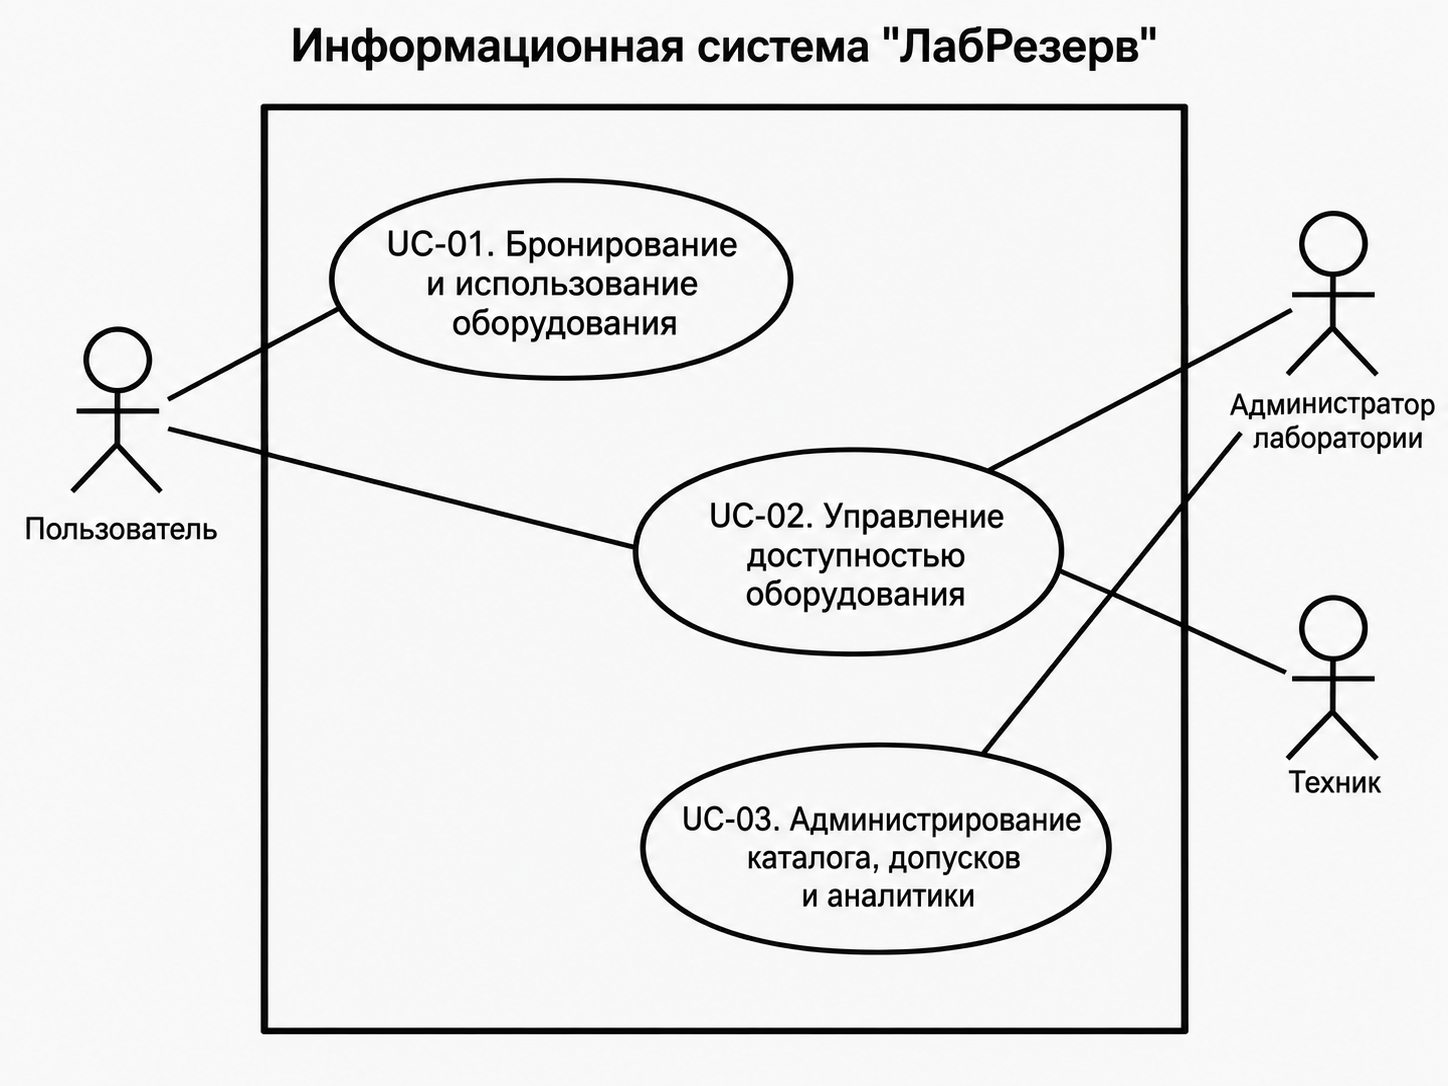
\includegraphics[width=0.96\textwidth,height=0.72\textheight,keepaspectratio]{usecase_overview.png}
\caption{Крупнозернистые прецеденты информационной системы \systemname}
\label{fig:usecases}
\end{figure}

\clearpage
\subsection{UC-01. Бронирование и использование оборудования}

На рисунке~\ref{fig:uc01-decomposition} показана декомпозиция UC-01. Основной
процесс включает просмотр каталога и календаря, создание бронирования и
фиксацию фактического использования. Разрешение конфликта подключается только
при недоступности исходного слота, а ручное согласование администратором ---
когда система не смогла подобрать подходящие альтернативы.

\begin{figure}[H]
\centering
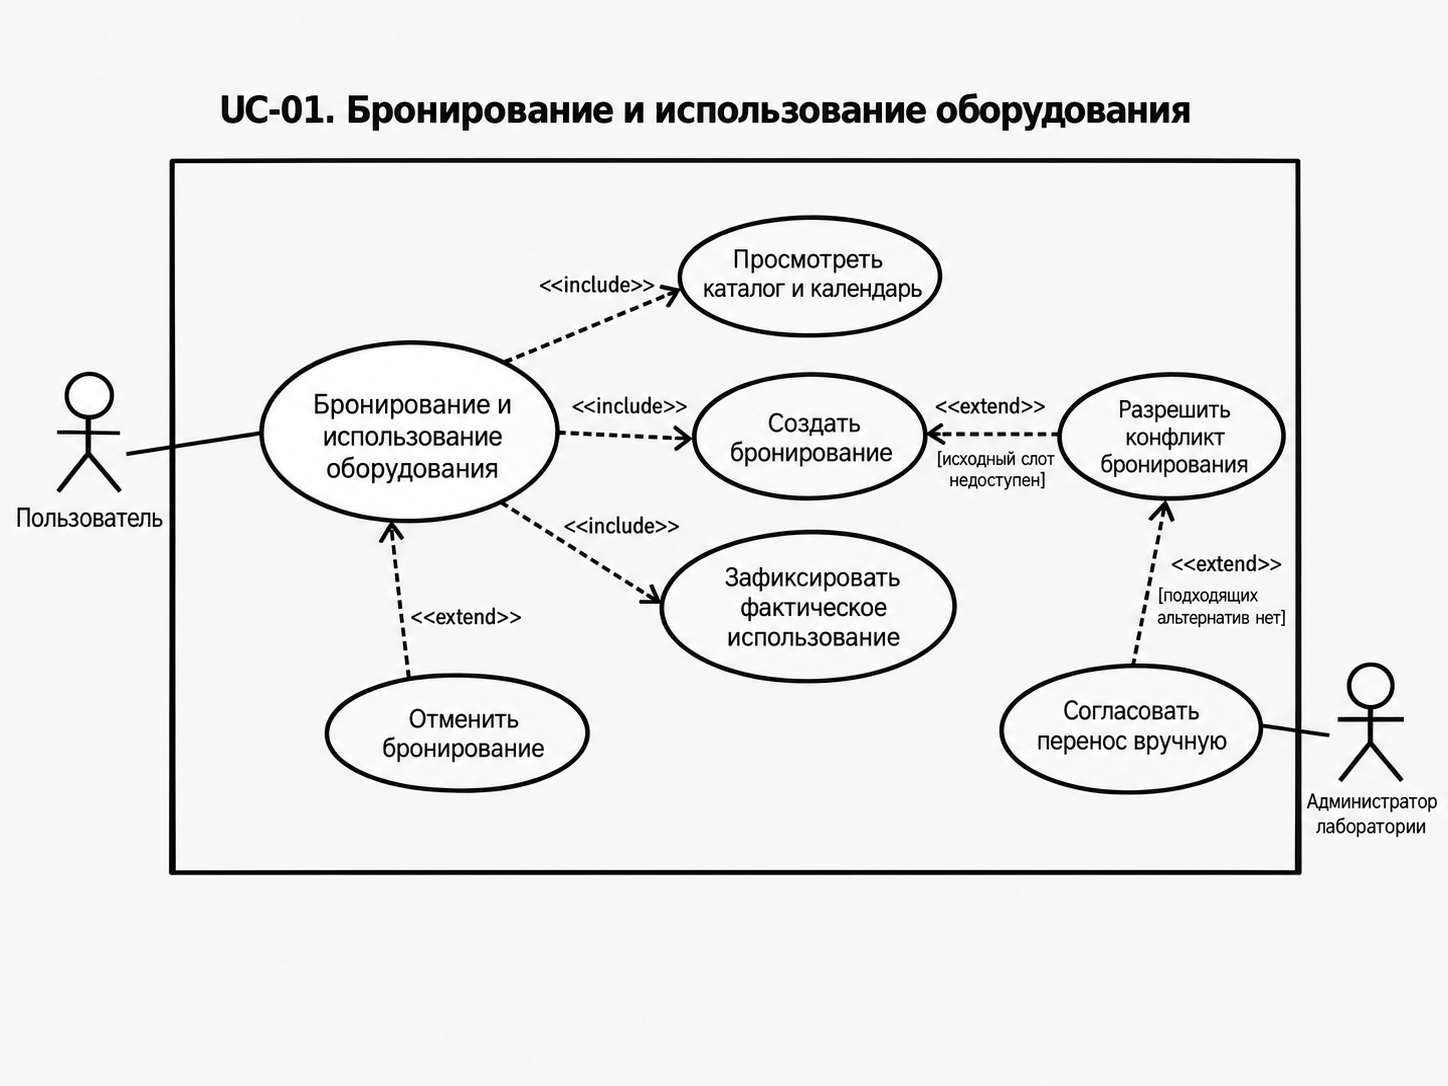
\includegraphics[width=0.96\textwidth,height=0.66\textheight,keepaspectratio]{usecase_uc01.png}
\caption{Декомпозиция UC-01 «Бронирование и использование оборудования»}
\label{fig:uc01-decomposition}
\end{figure}

\begin{longtable}{|p{0.25\textwidth}|p{0.65\textwidth}|}
\hline
Основные акторы & Пользователь; администратор лаборатории при ручном согласовании переноса. \\
\hline
Цель & Обеспечить полный цикл работы пользователя с оборудованием: найти подходящий
вариант, получить непротиворечивую бронь, выполнить работу и сохранить фактическое
использование. \\
\hline
Предусловия & Пользователь аутентифицирован и имеет действующую учётную запись;
оборудование присутствует в каталоге; сведения о допусках и доступности актуальны. \\
\hline
Основной сценарий &
\begin{ucsteps}
    \item Пользователь просматривает каталог, характеристики оборудования и календарь доступности.
    \item Пользователь выбирает оборудование или требуемую функцию, период и цель работы.
    \item Система проверяет допуск пользователя, техническое состояние оборудования, периоды обслуживания и пересечения с подтверждёнными бронированиями.
    \item Если исходный слот свободен, система повторно проверяет его в транзакции и создаёт подтверждённую бронь.
    \item Если исходный слот недоступен, система формирует и ранжирует допустимые альтернативы по времени и функционально эквивалентному оборудованию.
    \item Пользователь выбирает альтернативу, после чего система повторно проверяет её актуальность и переносит либо создаёт бронь.
    \item В назначенное время пользователь открывает фактический сеанс; система проверяет бронь, пользователя и текущее состояние оборудования.
    \item После завершения работы пользователь закрывает сеанс, а система сохраняет фактические начало, окончание и длительность отдельно от планового интервала.
    \item При необходимости пользователь отменяет будущее бронирование; отменённый интервал перестаёт блокировать расписание.
\end{ucsteps} \\
\hline
Альтернативы &
\begin{ucalts}
    \item У пользователя нет действующего допуска --- система отклоняет подтверждение и показывает причину.
    \item Допустимых автоматических альтернатив нет --- администратор лаборатории согласует перенос с пользователем вручную либо бронь остаётся в состоянии «требует переноса».
    \item Выбранная альтернатива стала недоступна из-за конкурентного запроса --- система пересчитывает список вариантов.
    \item До начала работы оборудование стало недоступно из-за ТО или неисправности --- бронь передаётся в UC-02 для обработки изменения доступности.
    \item Пользователь не завершил фактический сеанс --- администратор закрывает его с обязательным комментарием, действие фиксируется в аудите.
\end{ucalts} \\
\hline
Постусловия & Бронирование и фактический сеанс согласованы с допуском и текущей
доступностью оборудования; изменения отражены в расписании, уведомлениях и журнале аудита. \\
\hline
Связанные требования & FR-05--FR-13, FR-19--FR-21, FR-24; NFR-01--NFR-06. \\
\hline
\end{longtable}

\clearpage
\subsection{UC-02. Управление доступностью оборудования}

На рисунке~\ref{fig:uc02-decomposition} показана декомпозиция UC-02. Процесс
объединяет плановое обслуживание и обработку внеплановой неисправности, потому
что оба события меняют доступность оборудования и могут затронуть уже
существующие бронирования. В процессе участвуют пользователь, техник и
администратор лаборатории.

\begin{figure}[H]
\centering
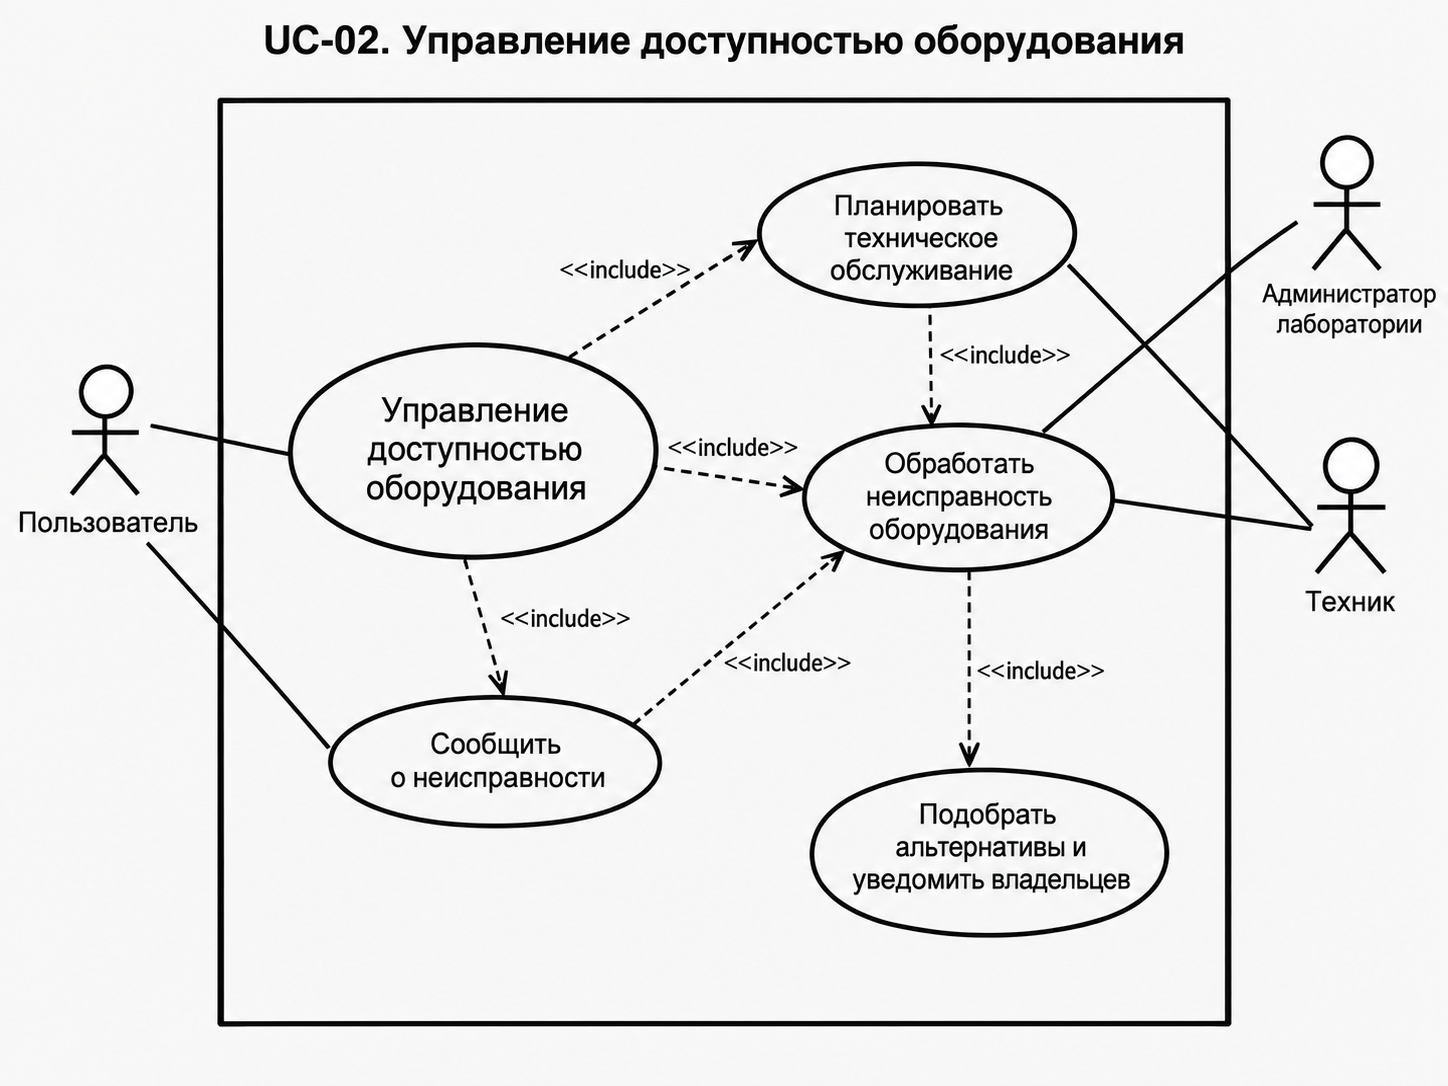
\includegraphics[width=0.96\textwidth,height=0.66\textheight,keepaspectratio]{usecase_uc02.png}
\caption{Декомпозиция UC-02 «Управление доступностью оборудования»}
\label{fig:uc02-decomposition}
\end{figure}

\begin{longtable}{|p{0.25\textwidth}|p{0.65\textwidth}|}
\hline
Основные акторы & Пользователь, техник, администратор лаборатории, владельцы затронутых бронирований. \\
\hline
Цель & Корректно изменить доступность оборудования при плановом обслуживании или
неисправности, обработать затронутые бронирования и вернуть оборудование в
эксплуатацию после завершения технических работ. \\
\hline
Предусловия & Оборудование существует и не архивировано; участники аутентифицированы;
в системе имеется актуальное расписание бронирований и технического состояния. \\
\hline
Основной сценарий &
\begin{ucsteps}
    \item Событие изменения доступности возникает одним из двух способов: техник планирует техническое обслуживание либо пользователь сообщает о признаках неисправности.
    \item При плановом обслуживании техник указывает оборудование, период, вид и содержание работ; система проверяет интервал.
    \item При неисправности система регистрирует сообщение и передаёт его технику и администратору для проверки.
    \item Техник или администратор подтверждает причину недоступности; система устанавливает соответствующее техническое состояние и блокирует период для новых бронирований.
    \item Система выявляет все затронутые будущие бронирования и переводит их в состояние «требует переноса».
    \item Система формирует и ранжирует допустимые альтернативы и уведомляет владельцев затронутых бронирований.
    \item Пользователи выбирают предложенные варианты; администратор контролирует случаи, для которых автоматический перенос невозможен.
    \item Система повторно проверяет выбранные интервалы и транзакционно обновляет расписание.
    \item Техник выполняет обслуживание или ремонт и фиксирует результат технических работ.
    \item После успешной проверки техник или администратор возвращает оборудование в состояние «доступно», если отсутствуют другие причины недоступности.
    \item Система обновляет календарь, уведомления и журнал аудита.
\end{ucsteps} \\
\hline
Альтернативы &
\begin{ucalts}
    \item Планируемый период пересекается с уже существующим обслуживанием --- техник изменяет границы периода.
    \item Сообщённая неисправность не подтверждена --- сообщение закрывается с заключением, состояние оборудования не изменяется.
    \item Для части затронутых броней нет допустимых альтернатив --- администратор согласует перенос или отмену вручную.
    \item Выбранная пользователем альтернатива стала недоступна --- система повторно рассчитывает варианты.
    \item Ремонт или обслуживание не завершены успешно --- оборудование остаётся недоступным, а технические работы продолжаются или переносятся.
\end{ucalts} \\
\hline
Постусловия & Причина недоступности и её период отражены в календаре; затронутые
бронирования обработаны или имеют явный статус; результат обслуживания или ремонта
сохранён в журнале. \\
\hline
Связанные требования & FR-14--FR-18, FR-21, FR-24; NFR-02, NFR-03, NFR-05, NFR-06. \\
\hline
\end{longtable}

\clearpage
\subsection{UC-03. Администрирование каталога, допусков и аналитики}

На рисунке~\ref{fig:uc03-decomposition} показана декомпозиция UC-03. Этот
прецедент объединяет административные действия, которые поддерживают остальные
сквозные процессы: ведение каталога оборудования, управление допусками,
получение сведений о техническом обслуживании и ремонтах, а также анализ
загрузки и выгрузку отчёта.

\begin{figure}[H]
\centering
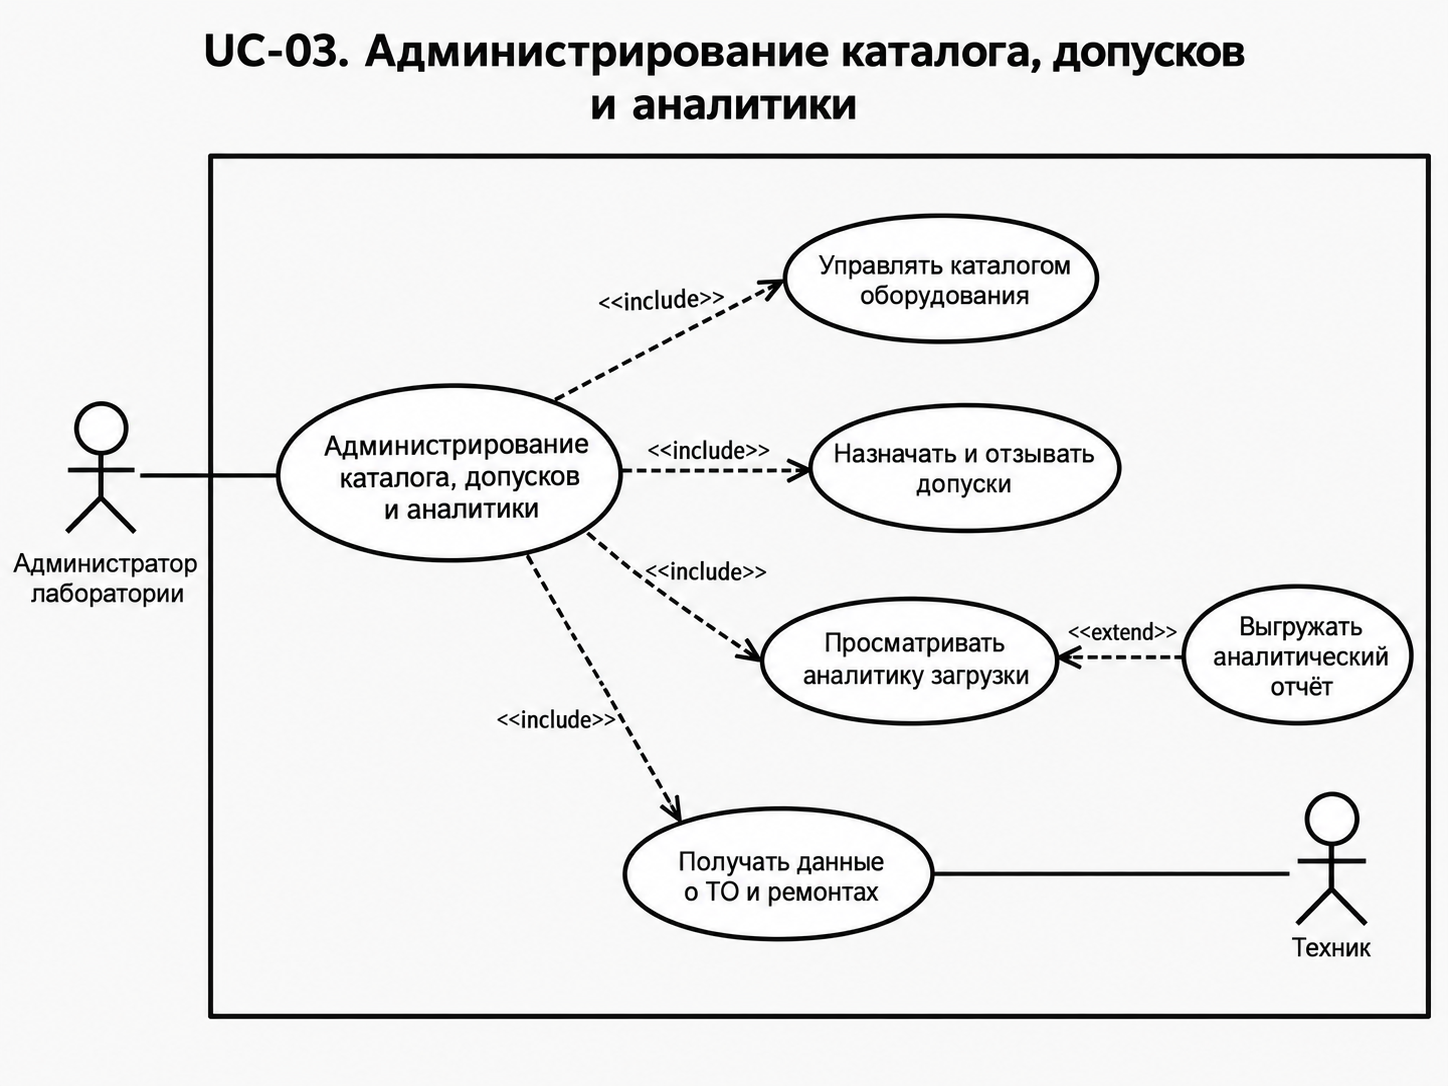
\includegraphics[width=0.96\textwidth,height=0.66\textheight,keepaspectratio]{usecase_uc03.png}
\caption{Декомпозиция UC-03 «Администрирование каталога, допусков и аналитики»}
\label{fig:uc03-decomposition}
\end{figure}

\begingroup
\small
\setstretch{1.15}
\renewcommand{\arraystretch}{1.1}
\begin{longtable}{|p{0.25\textwidth}|p{0.65\textwidth}|}
\hline
Основные акторы & Администратор лаборатории, техник. \\
\hline
Цель & Поддерживать достоверные справочные данные и права доступа, а также
получать аналитическую картину загрузки и недоступности оборудования. \\
\hline
Предусловия & Администратор аутентифицирован и имеет административные полномочия;
техник имеет право фиксировать результаты технических работ; прикладные данные
хранятся в системе. \\
\hline
Основной сценарий &
\begin{ucsteps}
    \item Администратор создаёт или изменяет типы и единицы оборудования, указывает характеристики, функции и требуемые виды допусков.
    \item Система проверяет целостность данных и сохраняет изменения каталога; использованное в истории оборудование вместо удаления архивируется.
    \item Администратор назначает, продлевает или отзывает допуски пользователей с указанием основания и срока действия.
    \item Система использует актуальные сведения о допусках при последующих проверках бронирований.
    \item Техник фиксирует сведения о техническом обслуживании и ремонтах; эти данные становятся частью истории доступности оборудования.
    \item Администратор задаёт период и фильтры аналитики по подразделению, типу или единице оборудования.
    \item Система рассчитывает плановую и фактическую загрузку, число конфликтов, длительность обслуживания, ремонтов и простоев.
    \item Система показывает агрегированные показатели и детализацию до связанных бронирований и технических событий.
    \item При необходимости администратор выгружает аналитический отчёт в CSV.
    \item Значимые административные изменения и факт выгрузки фиксируются в журнале аудита.
\end{ucsteps} \\
\hline
Альтернативы &
\begin{ucalts}
    \item Попытка удалить оборудование, которое уже использовано в истории, --- система предлагает архивирование вместо физического удаления.
    \item Срок допуска истёк --- новые бронирования по нему блокируются, а администратор получает возможность продлить или назначить новый допуск.
    \item Аналитических данных за выбранный период нет --- система показывает пустой результат без ошибки.
    \item Период или параметры отчёта заданы некорректно --- система предлагает исправить фильтры до расчёта или выгрузки.
\end{ucalts} \\
\hline
Постусловия & Каталог и допуски актуальны; сведения о технических работах доступны для
аналитики; сформированный отчёт соответствует выбранным фильтрам; изменения отражены в аудите. \\
\hline
Связанные требования & FR-02--FR-04, FR-18, FR-20, FR-22--FR-24; NFR-01, NFR-05, NFR-06. \\
\hline
\end{longtable}
\endgroup

\clearpage
\section{Архитектура системы}

\subsection{Архитектурный стиль}

Для первого релиза предлагается модульный монолит с трёхуровневой структурой:
веб-интерфейс, сервер приложений и реляционная база данных. Такой вариант
достаточен для ожидаемой нагрузки, упрощает транзакционную защиту расписания и
развёртывание на Helios. Границы модулей сохраняются в коде, поэтому при росте
нагрузки отдельные функции можно выделить в сервисы без преждевременного
усложнения проекта.

Клиент взаимодействует с сервером по REST/JSON. Серверная часть
собирается как WAR-приложение и развёртывается во внешнем сервере приложений
WildFly. Spring Boot в этой конфигурации используется как прикладной каркас и
точка конфигурации Spring, но не запускает встроенный веб-сервер: зависимость от
embedded Tomcat исключается, а Servlet/Jakarta Web-окружение предоставляет
WildFly. Статическая сборка React включается в WAR и раздаётся тем же
приложением.

На Helios предполагаются отдельный процесс WildFly с развёрнутым
\texttt{labreserve.war} и отдельный процесс PostgreSQL. Все серверные модули
реализуются как пакеты Java внутри одного WAR и работают в одном процессе
WildFly. Контроллеры, сервисы бизнес-логики и репозитории создаются и
связываются Spring IoC-контейнером; жизненным циклом веб-приложения,
HTTP-обработкой, пулом потоков и Servlet-окружением управляет WildFly.
Конкретные версии Spring Boot и WildFly необходимо подобрать совместимо с
доступной на Helios версией Jakarta Servlet API.

\subsection{Компоненты}

\begin{figure}[H]
\centering
\resizebox{0.98\textwidth}{!}{%
\begin{tikzpicture}[
    component/.style={draw,rounded corners,fill=lightblue,minimum width=3.8cm,
        minimum height=1.1cm,align=center,font=\small},
    store/.style={draw,cylinder,shape border rotate=90,aspect=0.3,
        fill=lightgray,minimum width=3.2cm,minimum height=1.4cm,align=center},
    flow/.style={-Latex,thick}
]
\node[component] (browser) at (0,4.8) {Веб-клиент\\React + TypeScript};
\node[component] (api) at (0,2.6) {REST API и безопасность\\Spring MVC + Spring Security};
\node[component] (booking) at (-5.8,0) {Модуль бронирований\\и конфликтов};
\node[component] (assets) at (0,0) {Модуль оборудования,\\допусков и обслуживания};
\node[component] (analytics) at (5.8,0) {Модуль аналитики\\и уведомлений};
\node[component] (data) at (0,-2.5) {Уровень доступа к данным\\Spring Data JPA + Hibernate};
\node[store] (db) at (0,-5) {PostgreSQL};
\node[draw,dashed,rounded corners,inner xsep=5mm,inner ysep=7mm,
    fit=(api)(booking)(assets)(analytics)(data)] (appcontainer) {};
\node[anchor=south east,align=right,font=\footnotesize]
    at ($(appcontainer.north east)+(-2mm,1mm)$)
    {Spring Boot: единый WAR\\Spring IoC в WildFly};

\draw[flow] (browser) -- node[right]{HTTPS, JSON} (api);
\draw[flow] (api) -- (booking);
\draw[flow] (api) -- (assets);
\draw[flow] (api) -- (analytics);
\draw[flow] (booking) -- (data);
\draw[flow] (assets) -- (data);
\draw[flow] (analytics) -- (data);
\draw[flow] (data) -- node[right]{SQL, транзакции} (db);
\end{tikzpicture}}
\caption{Компонентная архитектура системы}
\label{fig:components}
\end{figure}

\begin{itemize}
    \item \textbf{Модуль бронирований и конфликтов} проверяет ограничения,
    создаёт и переносит бронирования, а также формирует и ранжирует
    альтернативы.
    \item \textbf{Модуль оборудования, допусков и обслуживания} хранит каталог,
    функции, состояния и допуски, управляет плановыми работами,
    неисправностями и ремонтом.
    \item \textbf{Модуль аналитики и уведомлений} рассчитывает утилизацию,
    конфликтность и простой и формирует внутрисистемные уведомления. Его
    контракт допускает последующее подключение внешних каналов уведомления.
\end{itemize}

\subsection{Системная архитектура и размещение компонентов}

Системная архитектура показывает, где физически располагаются логические части
решения. На клиентском устройстве выполняется только браузер с React-интерфейсом.
На Helios размещаются входной reverse proxy, JVM с WildFly и развёрнутым
артефактом \texttt{labreserve.war}, а также PostgreSQL. Внутри WAR находятся
статическая React-сборка, REST-контроллеры, Spring Security, модули
бизнес-логики и слой JPA/Hibernate. Логические модули не запускаются как
отдельные процессы: они совместно используют Spring IoC-контейнер и одну
транзакционную инфраструктуру.

\begin{figure}[H]
\centering
\resizebox{0.96\textwidth}{!}{%
\begin{tikzpicture}[
    component/.style={draw,rounded corners,fill=lightblue,minimum width=4.4cm,
        minimum height=1.0cm,align=center,font=\small},
    store/.style={draw,cylinder,shape border rotate=90,aspect=0.3,
        fill=lightgray,minimum width=3.3cm,minimum height=1.4cm,align=center,font=\small},
    boundary/.style={draw,dashed,rounded corners,inner sep=7mm},
    flow/.style={-Latex,thick}
]
\node[component] (browser2) at (0,7.4) {Клиентское устройство\\Браузер + React/TypeScript};
\node[component] (proxy2) at (0,5.1) {Reverse proxy\\HTTPS-вход};
\node[component] (wildflyproc) at (0,2.9) {JVM + WildFly\\сервер приложений};
\node[component] (war2) at (0,0.7) {\texttt{labreserve.war}\\React static + REST + Security\\бизнес-логика + JPA/Hibernate};
\node[store] (db2) at (7.5,0.7) {PostgreSQL};

\node[boundary,fit=(wildflyproc)(war2),
    label=above right:{Процесс WildFly}] (wildfly2) {};
\node[boundary,fit=(proxy2)(wildfly2)(db2),
    label=above right:{Сервер Helios}] (helios2) {};

\draw[flow] (browser2) -- node[right]{HTTPS / 443} (proxy2);
\draw[flow] (proxy2) -- node[right]{HTTP, localhost} (wildflyproc);
\draw[flow] (wildflyproc) -- node[right]{deploy / execute} (war2);
\draw[flow] (war2) -- node[above]{JDBC / SQL, транзакции} (db2);
\end{tikzpicture}}
\caption{Системная архитектура и размещение компонентов}
\label{fig:system-architecture}
\end{figure}

\subsection{Выбор технологий}

\begin{longtable}{|p{0.23\textwidth}|p{0.25\textwidth}|p{0.42\textwidth}|}
\hline
\textbf{Уровень} & \textbf{Технология} & \textbf{Обоснование} \\
\hline
Клиент & React, TypeScript, Vite & Компонентный интерфейс календаря, строгая
типизация обмена и статическая производственная сборка. \\
\hline
Сервер & Java, Spring Boot, Spring MVC, Spring Security, WildFly &
Приложение собирается в WAR-файл и развёртывается во внешнем WildFly. Spring
обеспечивает REST, IoC, транзакции, валидацию и ролевую модель; embedded Tomcat
исключён из серверной конфигурации. \\
\hline
Доступ к данным & Spring Data JPA (Hibernate), JPQL и нативные запросы JPA &
JPA и Hibernate сокращают типовой код, а нативные запросы и вызовы процедур
PostgreSQL средствами JPA обеспечивают проверку интервалов и построение аналитики. \\
\hline
База данных & PostgreSQL & Поддерживает транзакции, ограничения, диапазонные
типы, индексы и серверные функции, необходимые на следующих этапах. \\
\hline
Миграции & Flyway & Версионируемое и воспроизводимое изменение схемы БД. \\
\hline
Тестирование & JUnit, Spring Boot Test, Testcontainers; Vitest & Проверка
бизнес-правил, SQL и клиентских компонентов в автоматизированной сборке. \\
\hline
\end{longtable}

Конкретные версии Java, Spring Boot, WildFly, Node.js и PostgreSQL необходимо
зафиксировать после проверки доступного окружения Helios и согласовать с
преподавателем до начала реализации.

\subsection{Развёртывание и окружение исполнения}

Диаграмма развёртывания отделяет физические узлы и процессы от логической
компонентной структуры. Пользователь работает на своём устройстве в браузере.
На узле Helios выполняются reverse proxy, JVM с WildFly и PostgreSQL. Артефакт
\texttt{labreserve.war} развёртывается внутри WildFly; отдельного процесса
Spring Boot или Tomcat нет.

\begin{figure}[H]
\centering
\resizebox{0.95\textwidth}{!}{%
\begin{tikzpicture}[
    nodebox/.style={draw,rounded corners,fill=lightgray,minimum width=4.5cm,
        minimum height=1.0cm,align=center,font=\small},
    proc/.style={draw,rounded corners,fill=lightblue,minimum width=5.0cm,
        minimum height=1.0cm,align=center,font=\small},
    artifact/.style={draw,rounded corners,fill=white,minimum width=4.5cm,
        minimum height=1.0cm,align=center,font=\small},
    host/.style={draw,dashed,rounded corners,inner sep=7mm},
    flow/.style={-Latex,thick}
]
\node[nodebox] (clientnode) at (-6,2.8) {Клиентское устройство};
\node[artifact] (browser) at (-6,0.9) {Браузер\\React + TypeScript};
\node[host,fit=(clientnode)(browser),label=above:{Узел пользователя}] (userhost) {};

\node[proc] (proxy) at (2.5,4.4) {Reverse proxy\\HTTPS :443};
\node[proc] (wf) at (2.5,1.9) {JVM + WildFly\\локальный HTTP-порт};
\node[artifact] (war) at (2.5,-0.3) {Артефакт \texttt{labreserve.war}\\React static, REST API, Security,\\сервисы, JPA/Hibernate};
\node[proc] (pg) at (2.5,-3.0) {PostgreSQL\\локальный TCP-порт};
\node[host,fit=(proxy)(wf)(war)(pg),label=above right:{Узел Helios}] (helios) {};

\draw[flow] (browser.east) -- node[above]{HTTPS} (proxy.west);
\draw[flow] (proxy) -- node[right]{HTTP / localhost} (wf);
\draw[flow] (wf) -- node[right]{развёртывание WAR} (war);
\draw[flow] (war) -- node[right]{JDBC / SQL} (pg);
\end{tikzpicture}}
\caption{Диаграмма развёртывания и окружение исполнения}
\label{fig:deployment}
\end{figure}

Сборка фронтенда помещается в статические ресурсы WAR-приложения. WAR-файл
развёртывается в WildFly, установленном на Helios. Для Spring Boot должна быть
использована WAR-конфигурация для внешнего Servlet-контейнера; встроенный Tomcat
не включается в итоговый артефакт. Параметры подключения к БД, ключи подписи и
профиль среды передаются через переменные окружения. Миграции Flyway применяются
при развёртывании приложения. Контейнеризация Docker/Podman и внешние облачные
сервисы для первого релиза не требуются.

\subsection{Обеспечение целостности и конкурентного доступа}

Проверка доступности выполняется как в прикладной логике, так и на уровне базы
данных. Создание брони происходит в транзакции. На следующем этапе следует
применить ограничение PostgreSQL, запрещающее пересечение активных временных
диапазонов для одной единицы оборудования, либо эквивалентную блокировку с
повторной проверкой. Благодаря этому два одновременных запроса не смогут
подтвердить один слот.

Изменение состояния оборудования, создание недоступности и пометка затронутых
броней выполняются одной транзакцией. Уведомления создаются в той же базе данных,
поэтому ошибка внешнего канала в будущем не приведёт к потере события.

\subsection{Безопасность}

Сервер проверяет аутентификацию, роль и принадлежность объекта для каждого
запроса. Пароли хранятся в виде адаптивных хешей, сессии или токены имеют
ограниченный срок жизни. Входные данные валидируются на границе REST API,
параметры SQL передаются безопасно. Журнал аудита недоступен для изменения через
пользовательский API. Секреты не включаются в исходный код и сборочные артефакты.

\section{Критерии приёмки первого этапа проектирования}

Результаты первого этапа считаются согласованными, если:

\begin{enumerate}
    \item преподаватель подтверждает границы предметной области и перечень
    основных акторов;
    \item прецеденты UC-01--UC-03 описывают сквозные процессы с участием
    нескольких ролей;
    \item для каждого функционального требования определён актор или системное
    событие, инициирующее функцию;
    \item нефункциональные требования имеют проверяемые критерии;
    \item выбранные версии Java, WildFly, Spring и PostgreSQL совместимы и
    доступны для демонстрации на Helios;
    \item отдельно согласованы приоритеты подбора альтернатив и правила
    обработки уже существующих броней при техническом обслуживании;
    \item архитектура допускает реализацию PostgreSQL-модели и серверных
    функций на следующих этапах.
\end{enumerate}

\section{Заключение}

На первом этапе описана предметная область управления лабораторным
оборудованием, определены назначение и границы системы, сформулированы
функциональные и нефункциональные требования. Построена модель основных
прецедентов с подробными сквозными сценариями бронирования и использования,
планового обслуживания, обработки поломок и восстановления расписания.

Предложена архитектура модульного монолита на основе React, Spring Boot,
WildFly и PostgreSQL. Серверная часть собирается в WAR и развёртывается на
Helios без встроенного Tomcat. Перед реализацией требуется подтвердить версии
технологий и правила ранжирования альтернатив для целевого окружения.

\end{document}
